\section{\large 結果と考察}
\subsection{レーン形成率の時間発展}
\par Fig. \ref{snapshot1},\ref{tvsphi}に各時刻におけるスナップショットとレーン形成率の時間発展を示す.$\tau$はシミュレーションでの時間単位である.このとき,外部電場$E_x=0.10$である.以下,デバイ長さは$\kappa^{-1}=10\Delta$で固定して計算を行った.
\begin{figure}[H]
\centering
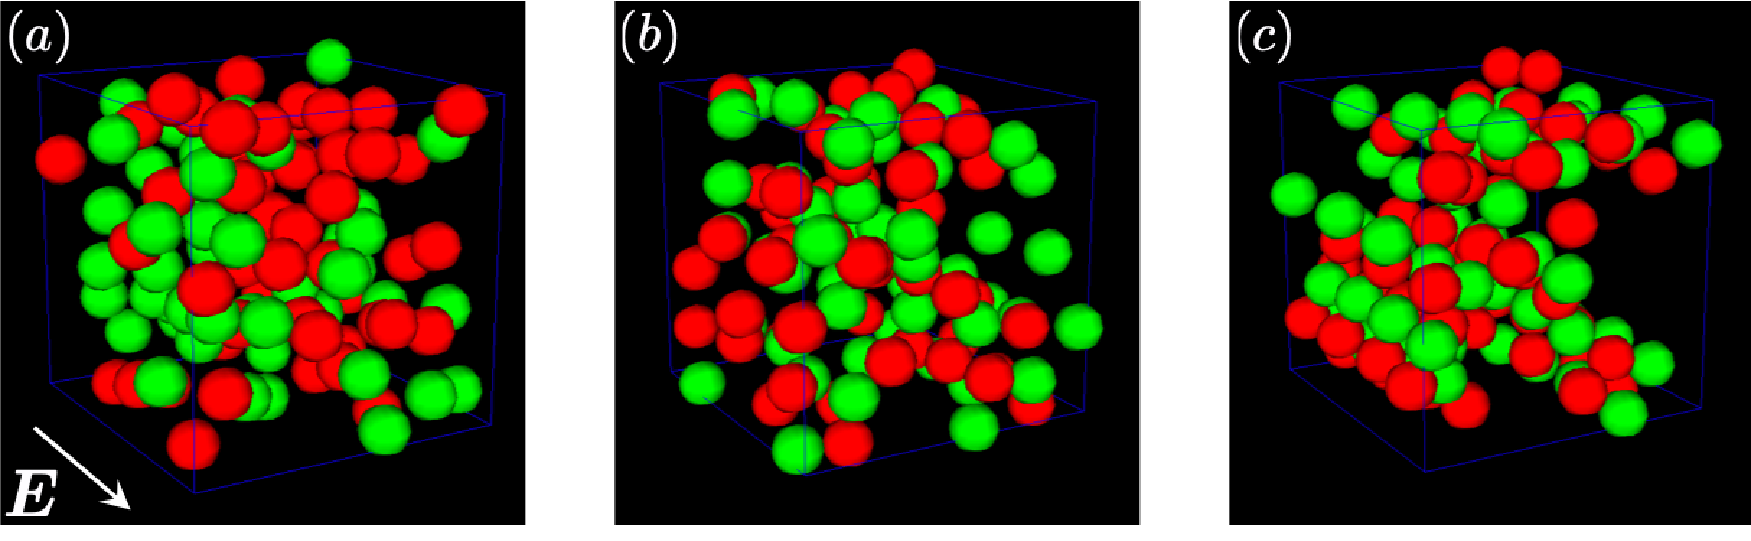
\includegraphics[scale = 0.5]{figures/snap1.pdf}
\caption{各時刻におけるスナップショット$(a)\, t/\tau=0$,$(b)\, t/\tau=3400$,$(c)\, t/\tau=18000$}
\label{snapshot1}
\end{figure}
%
%
\begin{figure}[H]
\centering
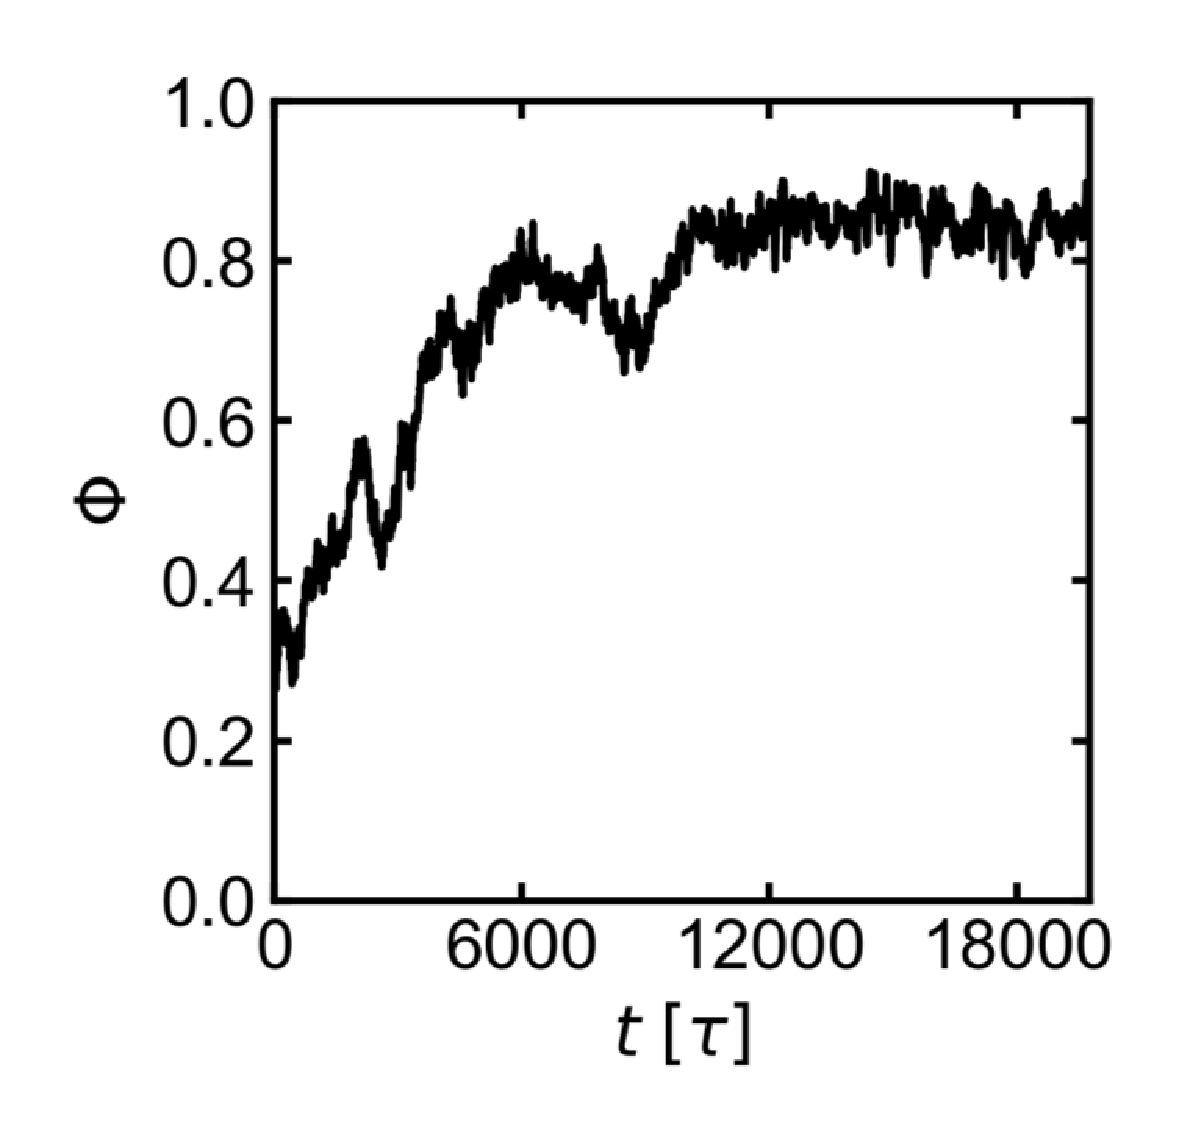
\includegraphics[width=8.0cm]{figures/tvsphi.pdf}
\caption{レーン形成率の時間発展}
\label{tvsphi}
\end{figure}
%
\noindent
Fig. \ref{snapshot1}の$(a)t/\tau=0$について,粒子の初期配置はランダムであり,このときのレーン形成率は$\Phi=0.28$である.
ランダムな粒子配置であっても$\Phi$は0.28程度の値を持つことに注意する.
$(b)t/\tau=3400$について,レーンが形成される途中の状態を表している.
レーンが形成される過程としては,対向する粒子が衝突した際に電場方向に垂直な方向に互いに押し出され,これを繰り返しながら同符号粒子が集合し整列する.
$(c)t/\tau=18000$について,レーンが形成されていることが確認できる.このとき,粒子配置は乱れることなく動き,系は定常状態へと達する.
\subsection{先行研究との比較}
\par 先行研究で用いられているペクレ数を用いて,比較を行った.
Fig. \ref{prework}が先行研究,Fig. \ref{EvsPhi}が今回のシミュレーションによる結果である.
\begin{figure}[H]
\centering
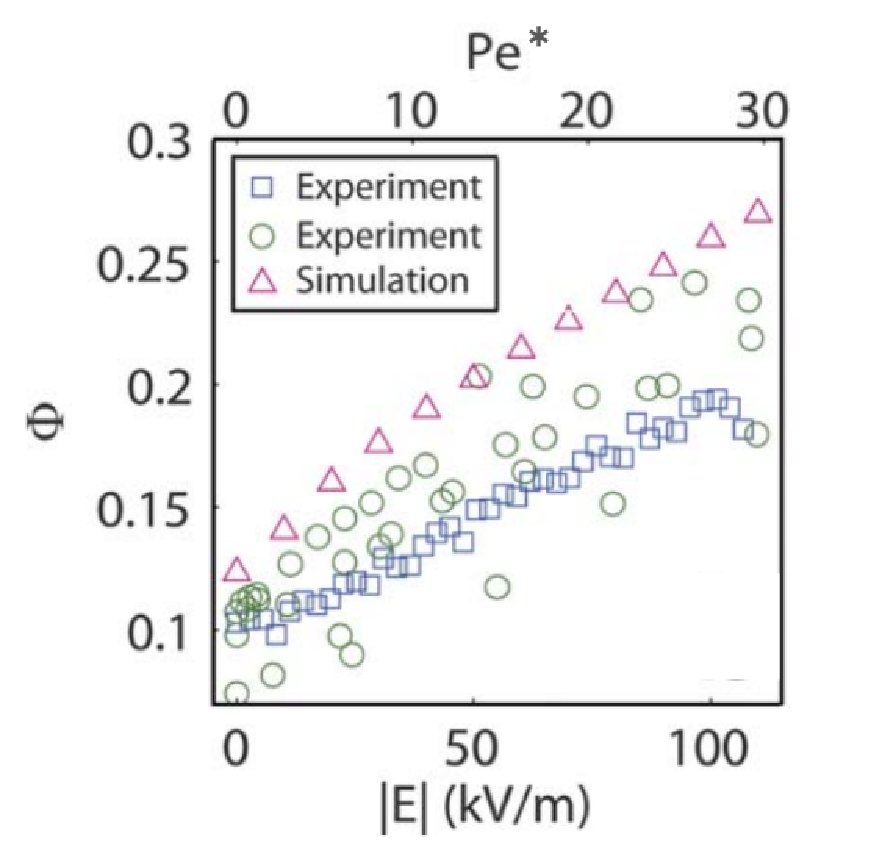
\includegraphics[width=9.1cm]{figures/EvsPhiPre.pdf}
\caption{先行研究におけるレーン形成率の電場依存性}
\label{prework}
\end{figure}
%
\begin{figure}[H]
\centering
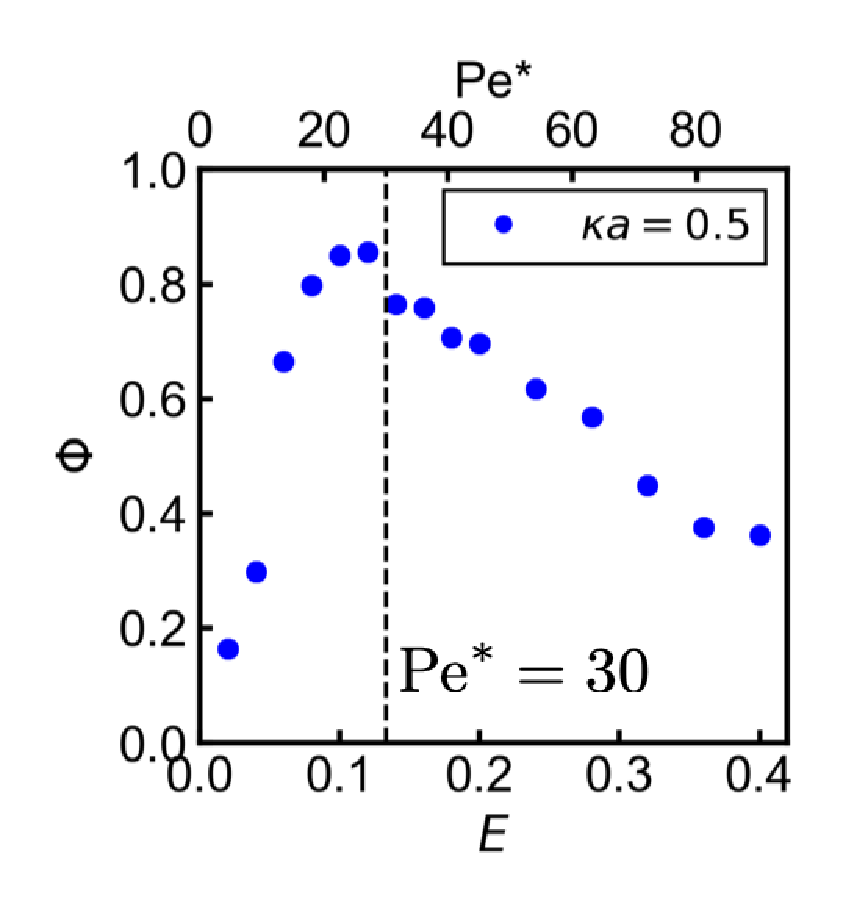
\includegraphics[width=8.0cm]{figures/EvsPhi.pdf}
\caption{本研究におけるレーン形成率の電場依存性}
\label{EvsPhi}
\end{figure}
%
\noindent
先行研究のグラフについて,緑の丸が瞬時に外部電場の大きさを変えた実験の結果,青の四角が徐々に外部電場を変化させた実験の結果,ピンクの三角が一定の外部電場をかけたときのシミュレーションの結果を表している.
先行研究でのレーン形成率と今回の研究でのレーン形成率の値が異なるのは,その定義の違いによるもので本質的な違いはない.
ここでペクレ数は以下の式で計算される.
$\boldsymbol{f}$は粒子が受ける力を表しており,$f(\kappa a)$はヘンリー係数である\cite{Henry}.
\begin{eqnarray}
	& \textrm{Pe}^* = \cfrac{|\textit{\textbf{f}}\,| a}{k_{\rm{B}} T}\\
	& \textit{\textbf{f}} = \cfrac{Ze\textit{\textbf{E}}f(\kappa a)}{1 + \kappa a}\\
	& f(\kappa a) = \cfrac{2}{3} \Biggl[1 + \cfrac{1}{2 \bigl(1 + \frac{2.5}{\kappa a (1 + 2 \rm{exp}(-\kappa a))}\bigl)^3}\Biggl]
\end{eqnarray}
Fig. \ref{prework}では,外部電場を大きくするほどレーン形成率が上昇していることが確認できる.
先行研究でのペクレ数の範囲をFig. \ref{EvsPhi}の破線で表し,対応させた.
Fig. \ref{EvsPhi}ではペクレ数が30以下の範囲では,レーン形成率は電場が大きくなるほど上昇しており,ペクレ数が30を超えると,レーン形成率が減少する傾向にあることが分かる.
先行研究のシミュレーションでは,ペクレ数が30を超えている領域でもレーンが形成されていくことが述べられているので,ペクレ数30を超えた領域では先行研究とは異なる振る舞いを見せることが分かった.
このレーン形成率の低下の原因について,次のように考えられる.
外部電場が大きくなり,粒子速度が速くなることで粒子配置を乱す流体力学的相互作用の影響が大きくなってくる.
この影響によって粒子配置に乱れが生じるようになり,粒子同士が安定なレーンを形成することができず,レーン形成率が低下すると推測される.

しかし,先行研究で用いられているペクレ数は,粒子が受ける力を外部電場からのみとして計算している.
今回のような正負混合多粒子系では,多体的な流体力学的相互作用や静電相互作用により粒子が受ける力を正確に見積もることは難しい.
そこで外部電場による駆動と拡散の比から,次の式でペクレ数を定義し直した.
ここで,$\bar{V}$は粒子の平均速度,$D_0$は拡散係数を表している.
\begin{eqnarray}
	& \textrm{Pe} = \cfrac{\bar{V}a}{D_0}  \label{Pe}\\
	& D_0 = \cfrac{k_{\rm{B}}T}{6 \pi \eta a}
\end{eqnarray}
%
Fig. \ref{PevsPhi}に式(\ref{Pe})で定義したペクレ数に対するレーン形成率を示す.

%
\begin{figure}[H]
\centering
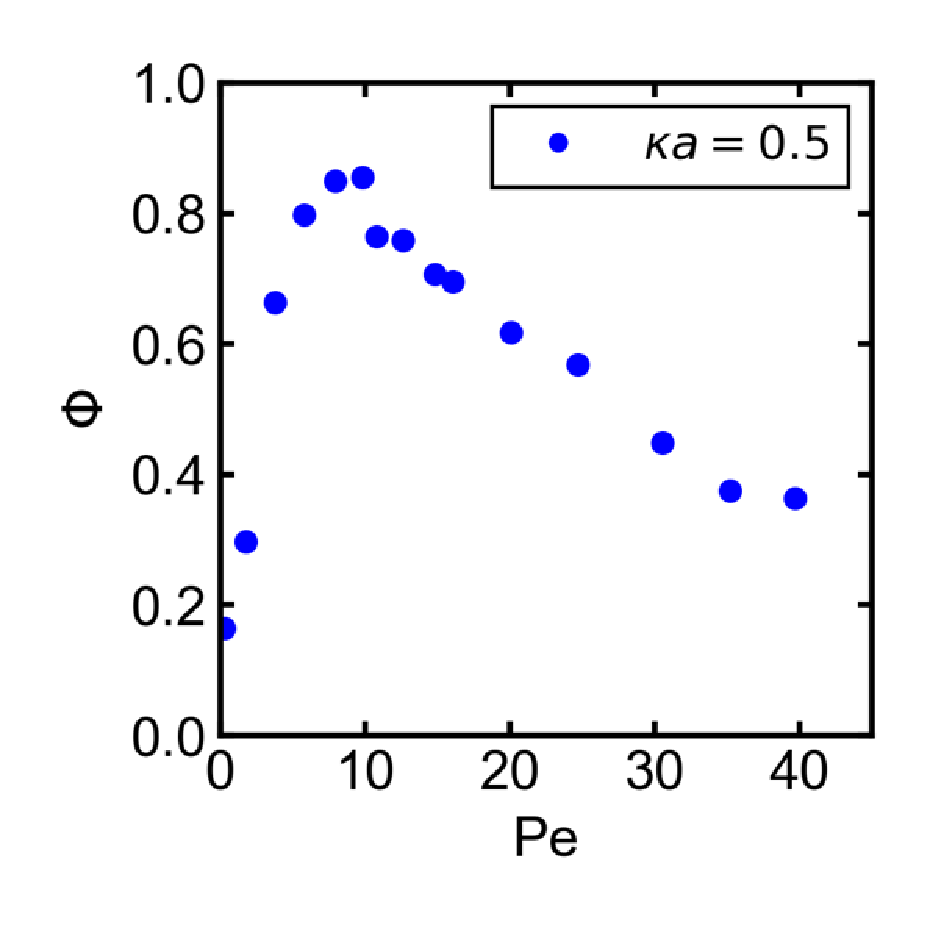
\includegraphics[width=8.0cm]{figures/PevsPhi.pdf}
\caption{レーン形成率のペクレ数依存性}
\label{PevsPhi}
\end{figure}
\noindent
ペクレ数を定義し直すことより,レーン形成率を定量的に評価した.
%
\subsection{レーン形成率の$\kappa a$依存性}
%
最後に液中のコロイド分散系において重要なデバイ長さとレーン形成率の関係について,$\kappa a=0.5,1.0,2.5$の場合をそれぞれ調べた.
\begin{figure}[H]
\centering
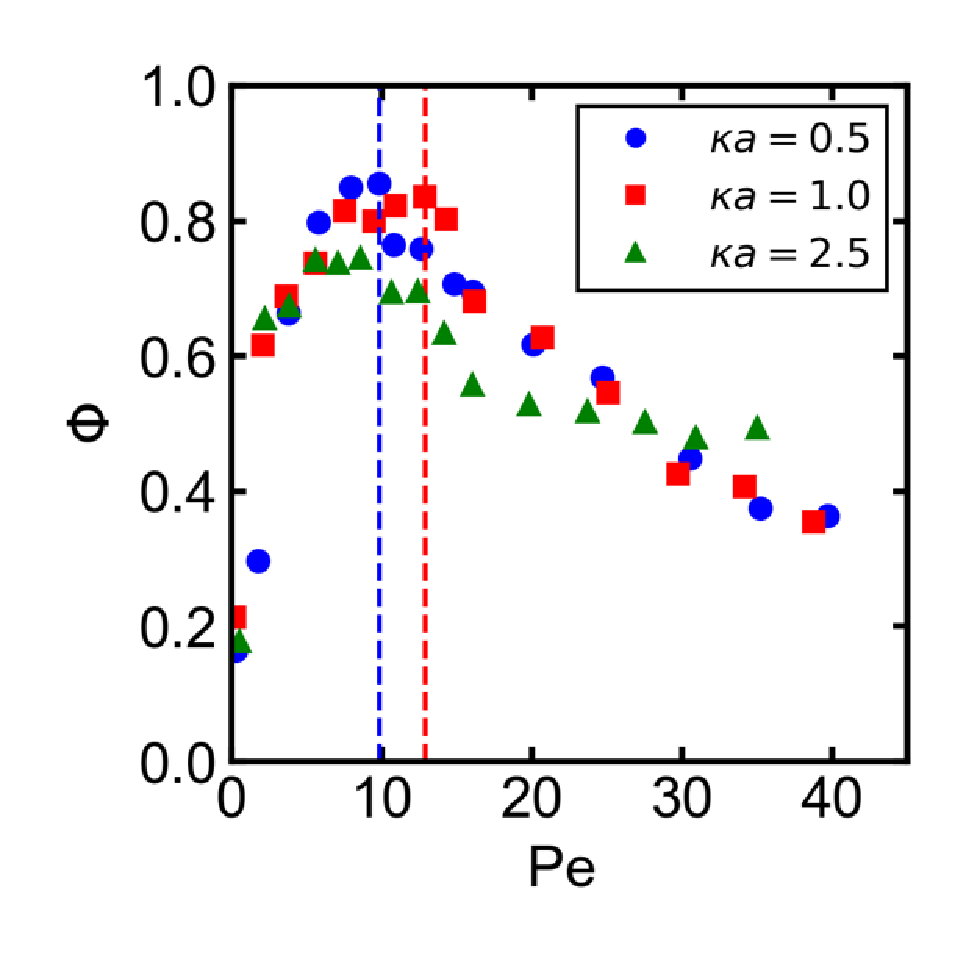
\includegraphics[width=8.0cm]{figures/kaPe2.pdf}
\caption{$\kappa a$とレーン形成率の関係}
\label{kaPhi}
\end{figure}
まず$\kappa a=0.5$と$\kappa a=1.0$の場合について述べる.$\kappa a$が大きいほど,つまりデバイ長さが小さいほどレーン形成率のピークが右にずれていることが分かる.
この傾向について,以下のように考えられる.コロイド粒子周りの電気二重層には粒子の表面電荷と反対符号の電荷を持つ電解質イオンが多く存在する.
電気二重層がコロイド粒子とは逆方向に力を受けることで,粒子周りにFig. \ref{ka2}の矢印のような流体の流れが生じ,他の粒子に影響を及ぼす.
しかし,この流れは電気二重層の厚みであるデバイ長さで減衰していくため,デバイ長さが小さいほど,つまり$\kappa a$が大きいほど電気二重層中の流れが及ぼす範囲が小さなり,他の粒子に影響を及ぼさなくなる.
この相互作用の影響が$\kappa a=1.0$のときには$\kappa a=0.5$のときと比べ小さくなるため,より大きなペクレ数まで安定したレーンが形成されていったと考えられる.
\begin{figure}[H]
\centering
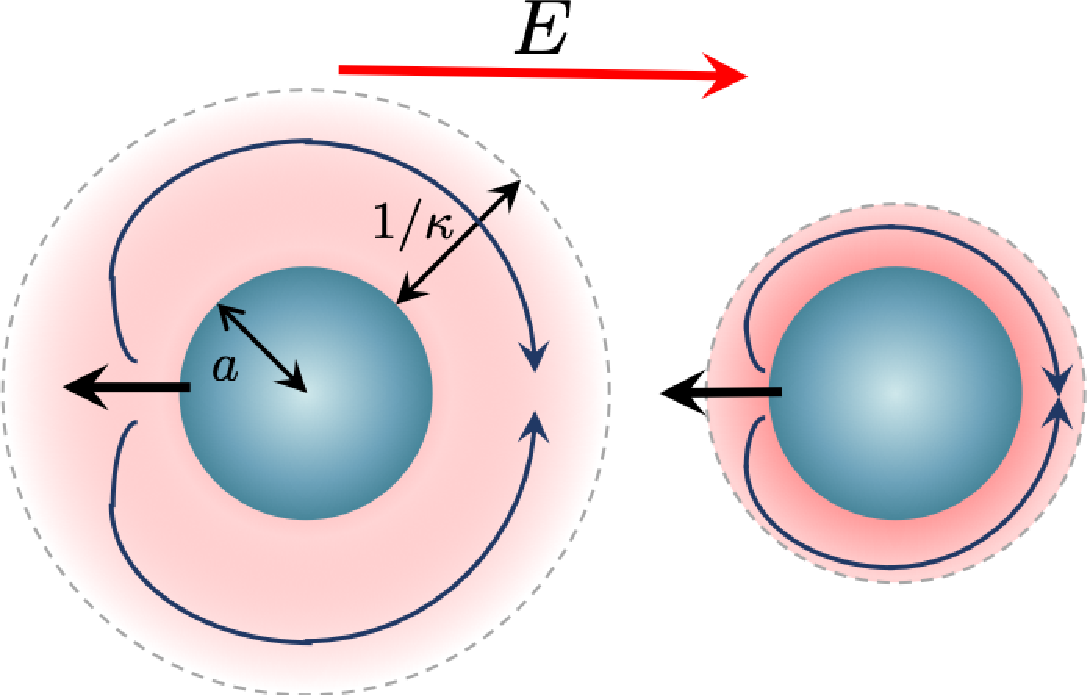
\includegraphics[width=8.0cm]{figures/ka2.pdf}
\caption{電気二重層中の流れ.左が$\kappa a$が小さい場合,右が$\kappa  a$が大きい場合を表す.}
\label{ka2}
\end{figure}
\noindent
ただし,$\kappa a=2.5$の場合にはこの傾向から外れていることが確認できる.この原因について次のように考えられる.$\kappa a=2.5$ではデバイ長さが$2\Delta$となり,グリッド幅に近づく.そのため,シミュレーションボックスの格子上に十分なデータが無くなり,計算が不安定化していると考えられる.
%
%
%
%
%
%
%
%
%
%
%
%
%
%
%
